\message{ !name(paper.tex)}\documentclass[10pt,twocolumn,letterpaper]{article}

\usepackage{cvpr} \usepackage{times} \usepackage{epsfig}
\usepackage{graphicx} \usepackage{amsmath} \usepackage{amssymb}
\usepackage{subfig}

% Include other packages here, before hyperref.

% If you comment hyperref and then uncomment it, you should delete
% egpaper.aux before re-running latex.  (Or just hit 'q' on the first
% latex run, let it finish, and you should be clear).
\usepackage[pagebackref=true,breaklinks=true,letterpaper=true,colorlinks,bookmarks=false]{hyperref}


% \cvprfinalcopy % *** Uncomment this line for the final submission

\def\cvprPaperID{****} % *** Enter the 3DIMPVT Paper ID here
\def\httilde{\mbox{\tt\raisebox{-.5ex}{\symbol{126}}}}

% Pages are numbered in submission mode, and unnumbered in
% camera-ready
\ifcvprfinal\pagestyle{empty}\fi
\begin{document}

\message{ !name(paper.tex) !offset(200) }
\begin{figure}
  \centering
  \subfloat[][]{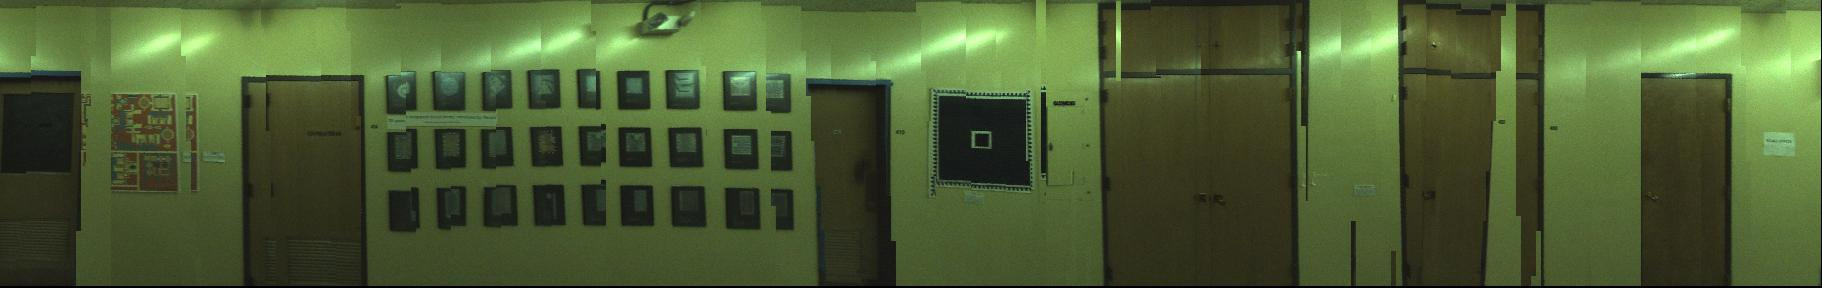
\includegraphics[width=3in, clip=true]{wall1_naive.jpg}}

  \centering
  \subfloat[][]{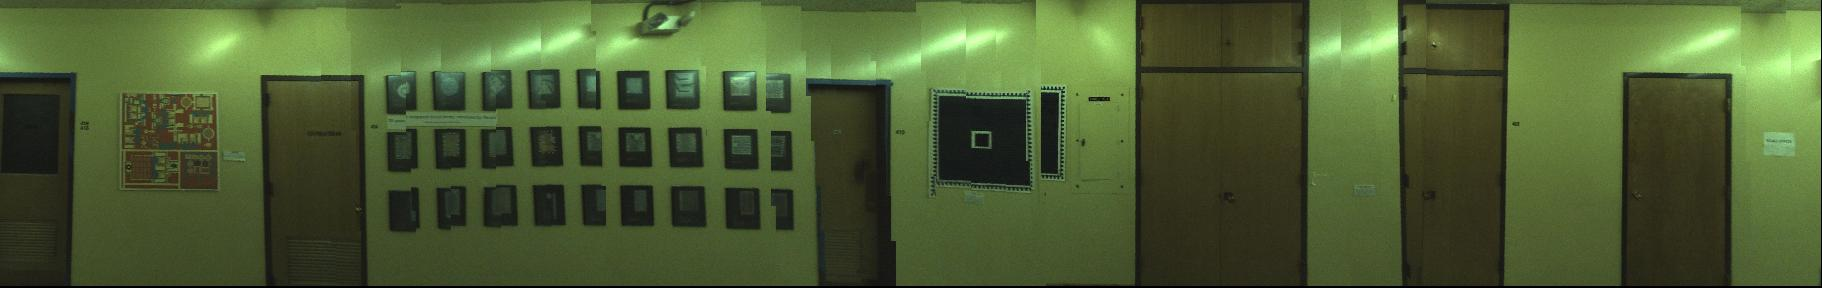
\includegraphics[width=3in, clip=true]{wall1_cache.jpg}}

  \centering
  \subfloat[][]{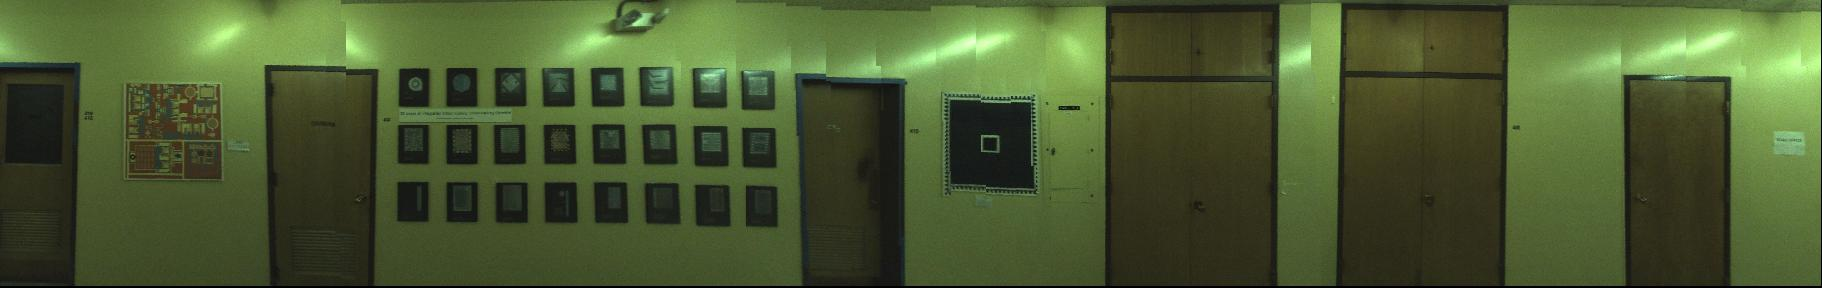
\includegraphics[width=3in, clip=true]{wall1_cache_shift.jpg}}

  \centering
  \subfloat[][]{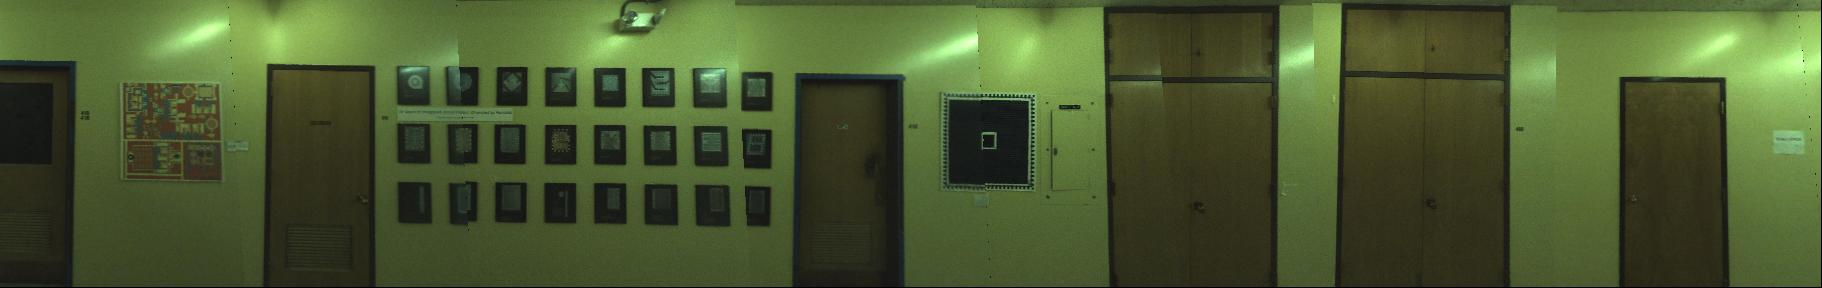
\includegraphics[width=3in, clip=true]{wall1_dynprog_noblend.jpg}}

  \centering
  \subfloat[][]{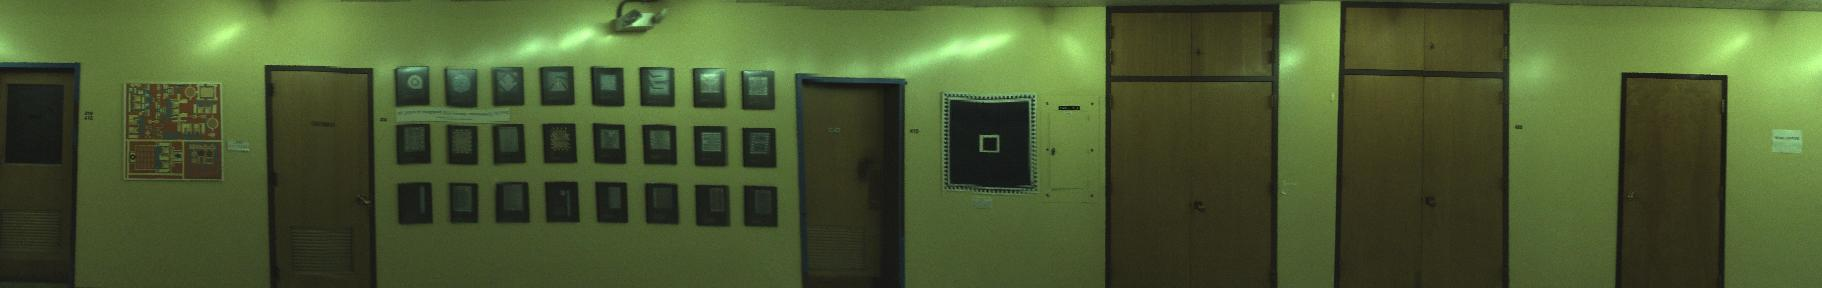
\includegraphics[width=3in, clip=true]{wall1_cache_shift_blend.jpg}}

  \centering
  \subfloat[][]{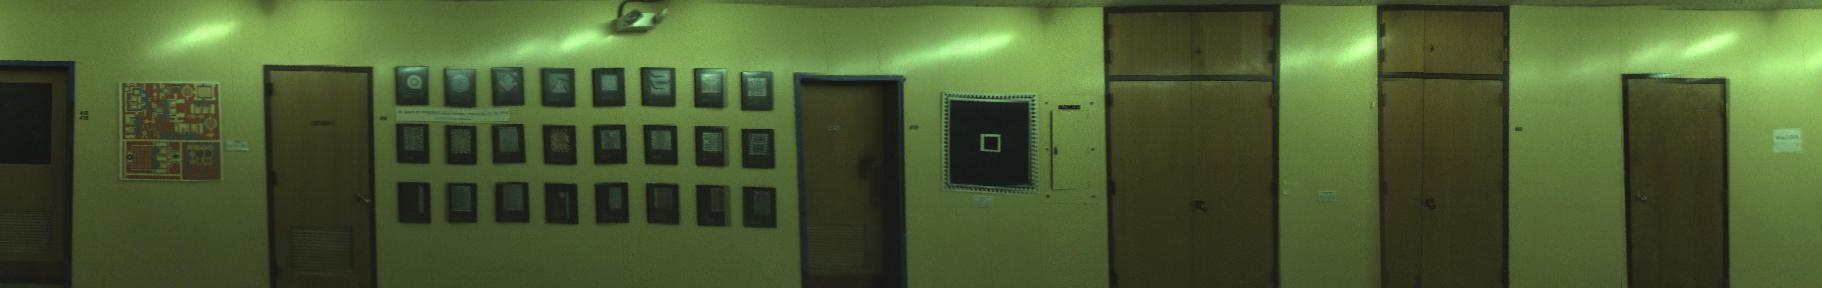
\includegraphics[width=3in, clip=true]{wall1_dynprog.jpg}}
  \caption{(a) Direct mapping. (b) Mapping with caching. (c) Mapping
    with caching after image alignment. (d) Seam minimization after
    image alignment). (e) same as (c) with blending. (f) same as (d)
    with blending.}
  \label{fig:compareAll}
\end{figure}
\message{ !name(paper.tex) !offset(715) }

\end{document}
